\section{Klasterovanje}
\label{sec:Klasterovanje}

Isprobali smo razli\v{c}ite algoritme klasterovanja. Po\v{c}etna ideja je bila da na taj na\v{c}in izdvojimo grupe pesama koje su sli\v{c}ne i prema tome formiramo liste pesama. Ovu ideju smo sproveli algoritmima K-sredina, K-medioida, DBSCAN i algoritmom hijerarhijskog klasterovanja. Medjutim, dobijeni rezultati nisu bili zadovoljavaju\'c{}i te ne\'c{}emo ulaziti u njihovu dublju analizu.

Na slici \ref{fig:knime-klasterovanje} prikazan je KNIME workflow koji smo koristili za isprobavanje algoritama.

\begin{figure}[H]
\centering
    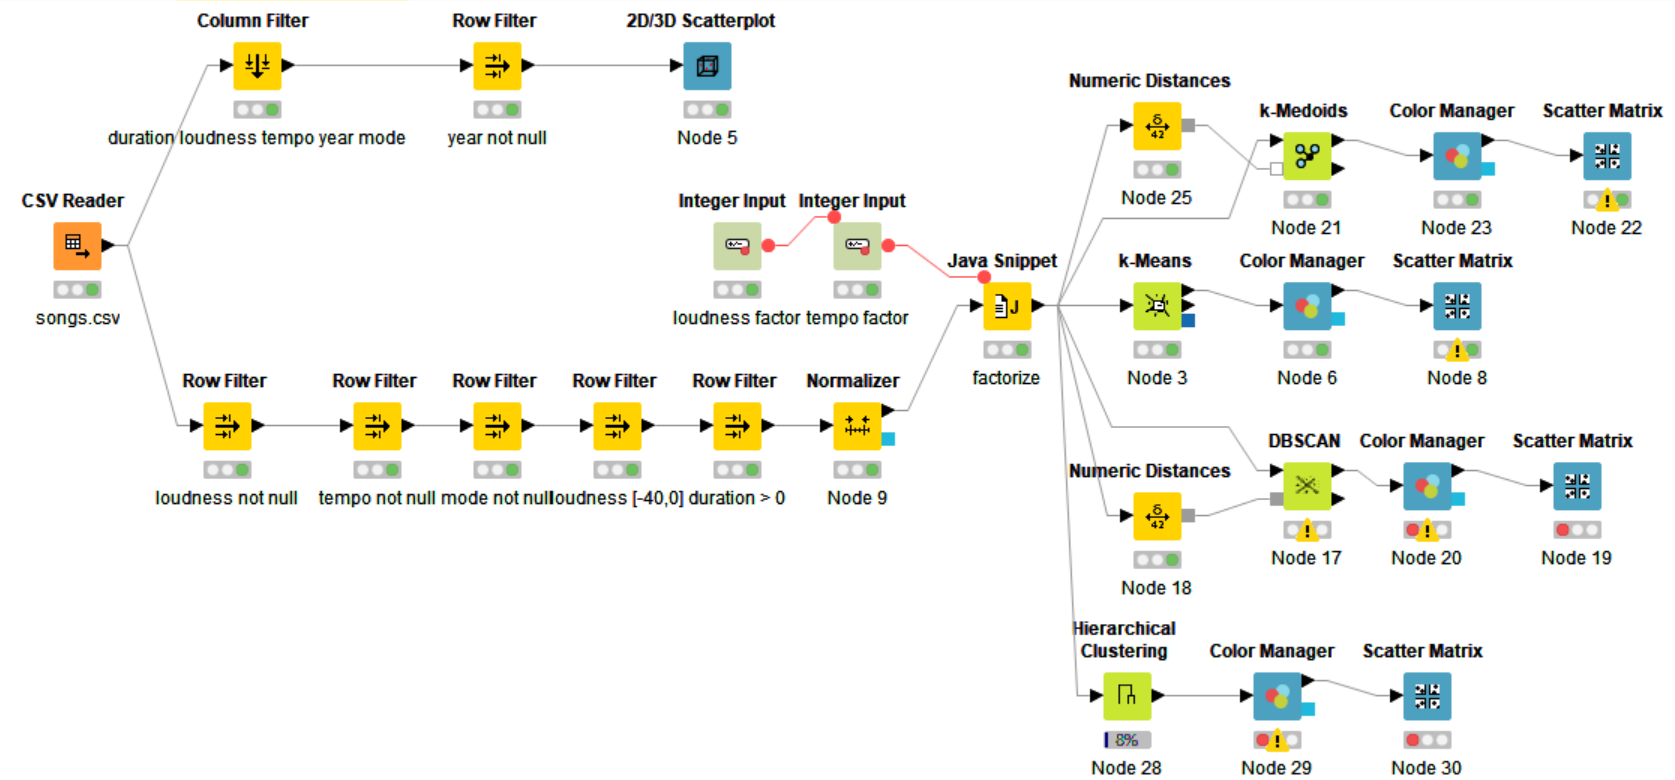
\includegraphics[scale=0.5]{KNIME workflows/screenshots/klasterovanje.PNG}
    \caption{KNIME workflow klasterovanje}
    \label{fig:knime-klasterovanje}
\end{figure}


